\chapter{Analyse}

\section{Ist Situation}
In der Vorgängerarbeit \enquote{Cygnet} von Stefan Rohner und Marco
Tanner\cite{cygnet:2013} wurde der Policy Server \enquote{strongTNC}
implementiert. Das Produkt und die Codebasis dieser Arbeit dient als Grundlage
für diese Arbeit.\\
Im Bereich des SWID Generators gibt es zur Zeit noch keine bestehenden Produkte.

\subsection{Stand der strongTNC Webapplikation} 
strongTNC ist eine Umsetzung des TNC Policy Servers, implementiert wurde dieser
als Webapp mit dem Python basierten \enquote{Django Web Framework} in Version
1.6\footnote{\url{https://www.djangoproject.com/}}. Die Applikation bietet
Unterstützung für das Verwalten von Geräten, Policies, Enforcements und erlaubt
es die Anwendung der Enforcements mittels hierarchischer Gruppen zu steuern.
Stammdaten wie Dateien oder Softwarepakete und Messresultate können eingesehen
und teilweise bearbeitet werden. Für SWID Tags besteht derzeit keine
Unterstützung, allerdings wurden bereits Views für SWID Tags und Regids
erstellt, diese haben jedoch keine Funktionalität und dienen gewissermassen als
Vorschau für zukünftige Features. \\ Im Frontend der Webapplikation wurden
Bootstrap 2.3\footnote{\url{http://getbootstrap.com/2.3.2/}} sowie jQuery
1.9\footnote{\url{http://jquery.com/1.9}} eingesetzt. Grundsätzlich werden die
Ansichten als \enquote{Master-Detail View} dargestellt. Als Schnittstelle zur
strongSwan IPsec Infrastruktur dient eine gemeinsam genutzte
SQLite\footnote{\url{http://www.sqlite.org/}} Datenbank.

Django Webapplikationen lassen sich in Module, sogenannte \enquote{Apps},
aufteilen, diese Möglichkeit wird allerdings nicht genutzt wie man dem Diagramm
der Applikation (\autoref{django-ist-diagram}) entnehmen kann. Die Django-Models
sind sehr eng an das Datenbankschema angelehnt, es ist gängig, dass die
Datenbank aus den Models generiert wird, dadurch wird die Datenbank für den
Entwickler vollständig abstrahiert. Da die Datenbank als Schnittstelle dient und
darum nicht ausschliesslich von Django verwendet wird, kann dieses Feature nicht
genutzt werden. Das Datenbankschema der bestehenden Tabellen, inklusive der
Erweiterung, ist in \autoref{fig:database-model} abgebildet.

\subsection{Architektur}
In \autoref{django-ist-diagram} ist eine Grobübersicht über die Architektur der
Involvierten Komponenten ersichtlich.

\begin{figure}[H]
	\centering
	\includegraphics[width=\textwidth]{images/architecture/django_apps_ist}
    \caption{Monolithische Django App}
    \label{django-ist-diagram}
\end{figure}

Den Ablauf einer Messung kann man dem folgenden Sequenzdiagramm,
\autoref{architecture-sequence-diagramm}, entnehmen:
\begin{figure}[H]
	\centering
	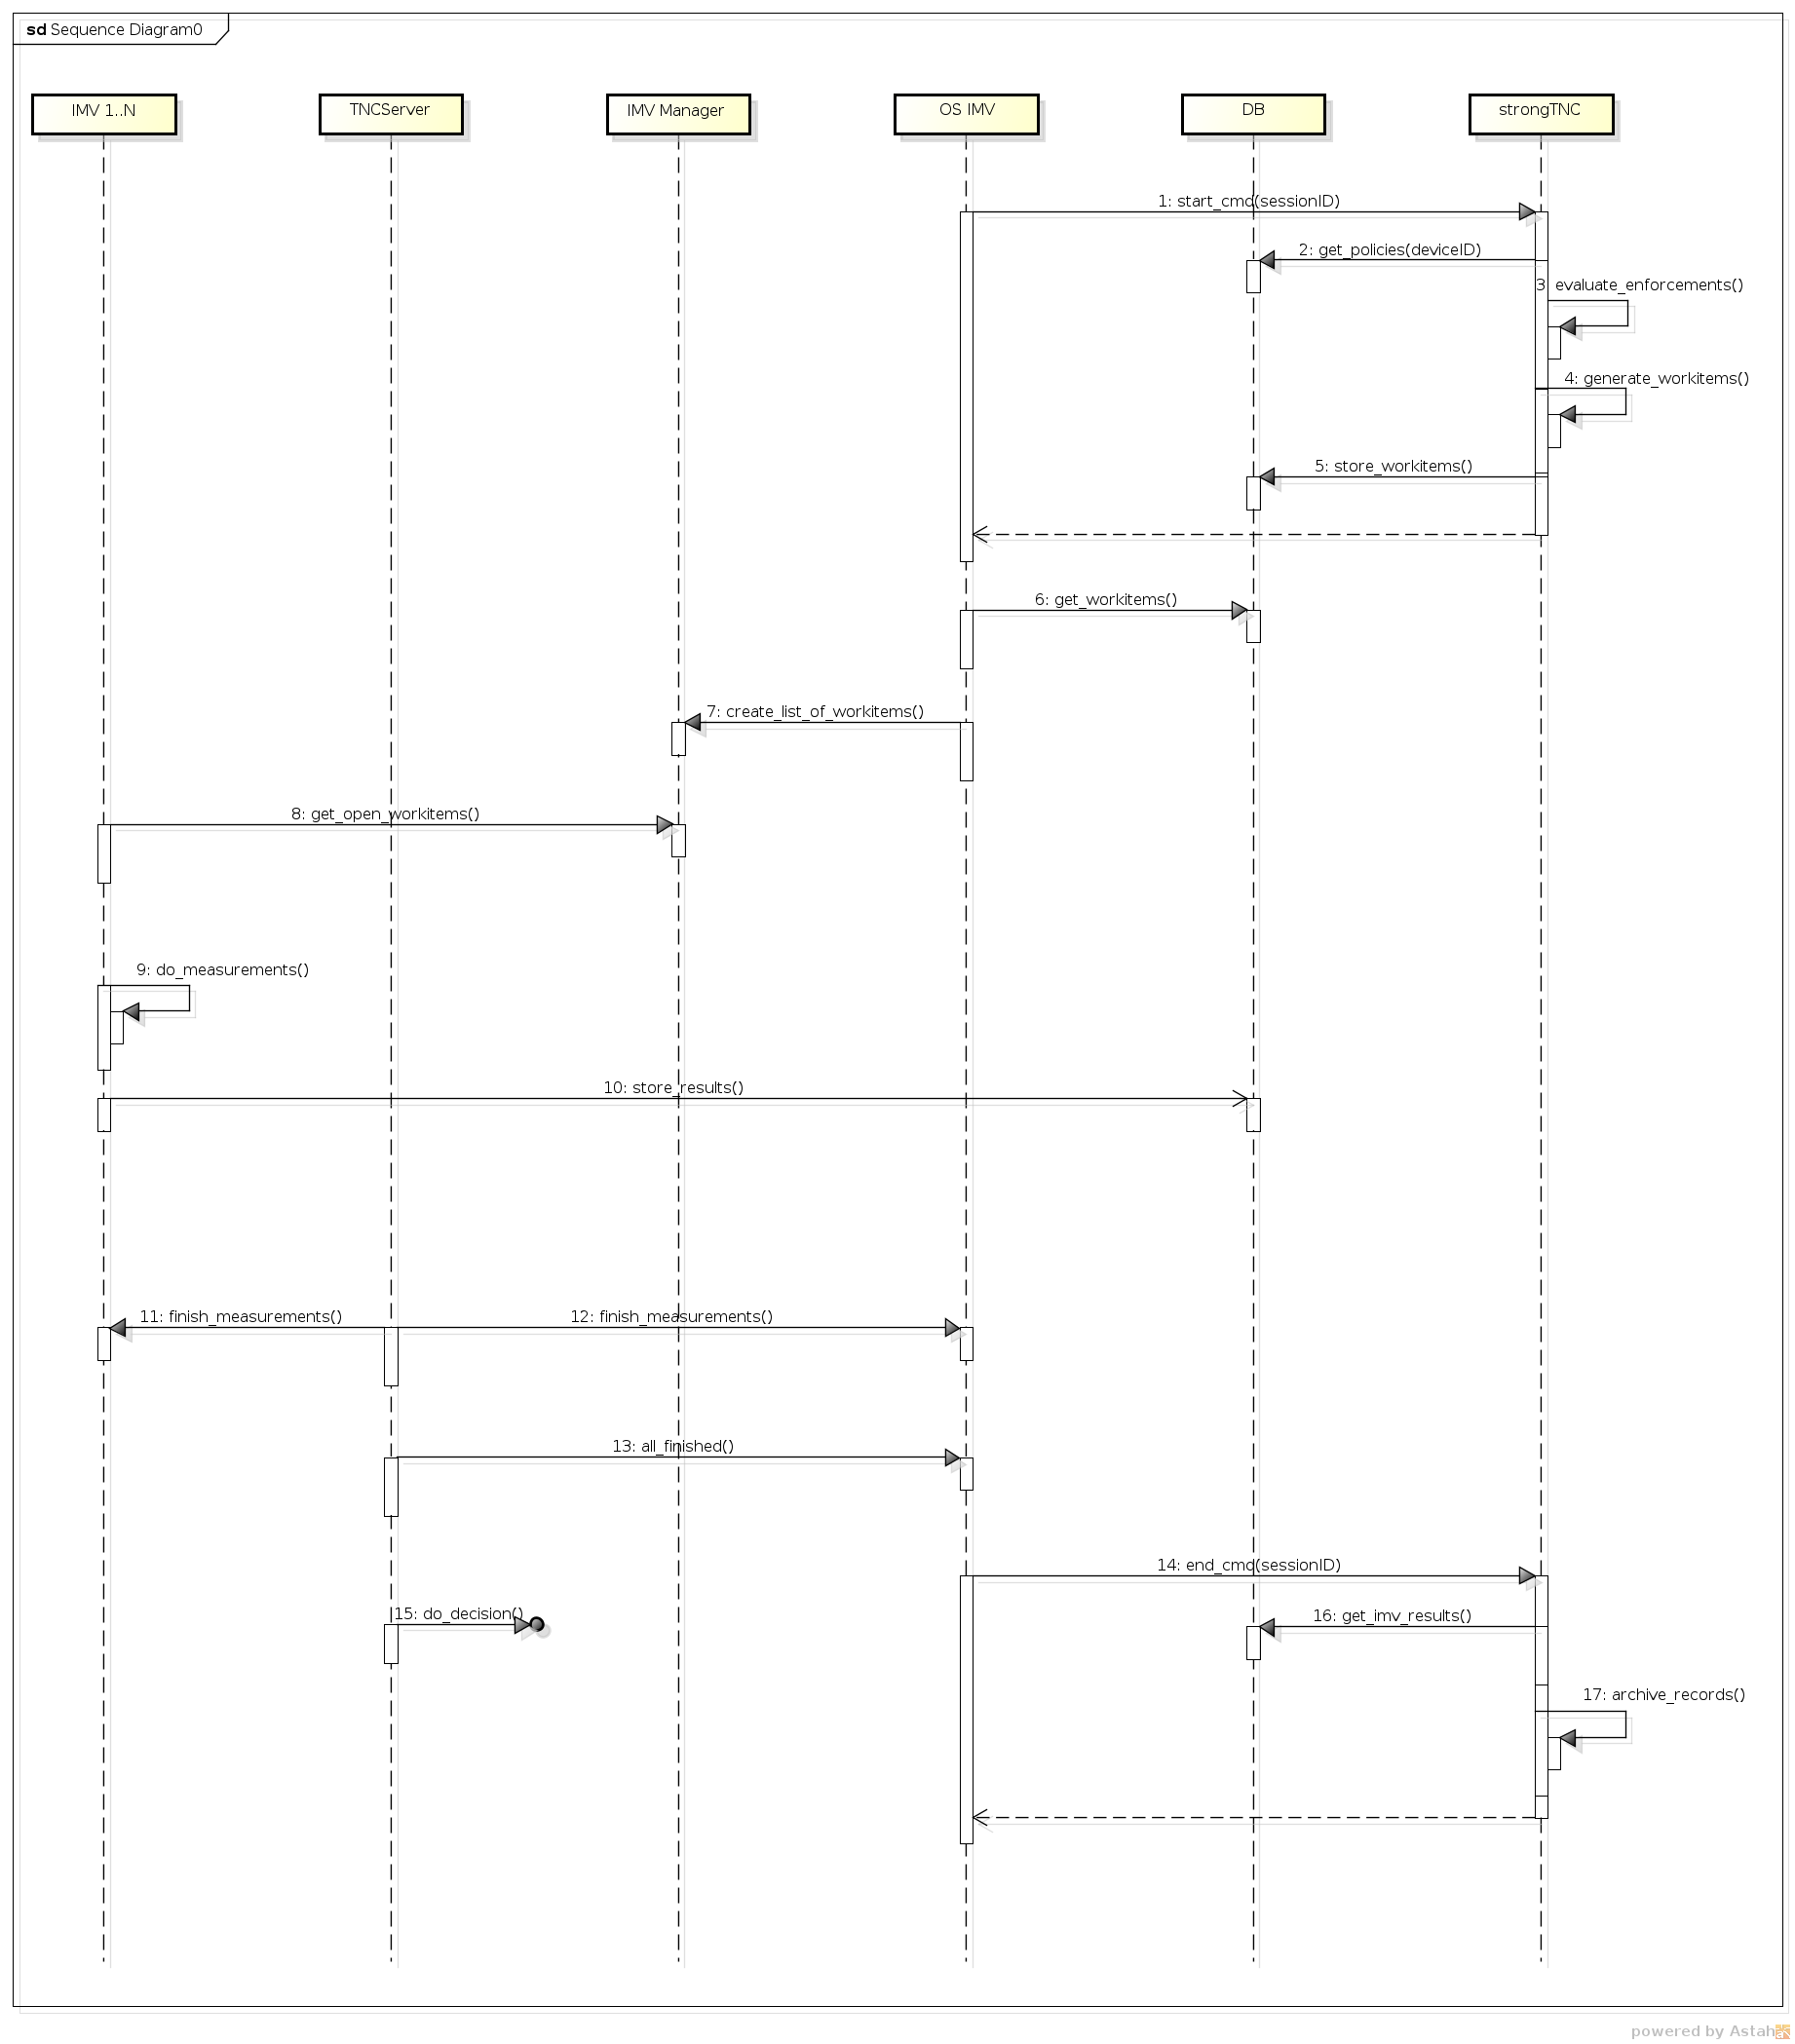
\includegraphics[width=\textwidth]{./images/architecture/architecture_sequence_diagramm-2014-03-12}
	\caption{}
	\label{architecture-sequence-diagramm}
\end{figure}

Laut dem technischen Bericht der der Vorgängerarbeit
\enquote{Cygnet}\cite{cygnet:2013} sollen die Richtlinien des \enquote{Style
Guide for Python Code}\cite{PEP8:2001}, genannt PEP8, eingehalten werden. Es
existieren elf Unit-Tests welche den bestehenden Python Code zu 21\% abdecken.\\


\subsubsection{Einschätzung}
\begin{description}
	\item[Ergänzungen] Es existiert noch keine Möglichkeit zur Erfassung und
	Verwaltung von SWID Tags, diese müssen im Rahmen dieser Arbeit erstellt werden.
	Die bestehenden Views können gegebenenfalls als Vorlage verwendet werden.
	
	\item[Schnittstelle] Das Verwenden einer gemeinsamen Datenbank stellt in unseren
	Augen ein Architekturproblem dar, welches dringend angegangen werden muss.
	Einerseits wird die Interoperabilität mit anderen Systemen stark eingeschränkt,
	andererseits wird die Wartbarkeit und Ausbaufähigkeit aller beteiligten
	Komponenten erschwert oder verunmöglicht. In diesem Fall wird ausserdem SQLite
	als Datenbank verwendet. SQLite ist nur bei lesendem Zugriff mehrbenutzerfähig,
	bei schreibendem Zugriff wird die Datenbank gesperrt, da eine gemeinsam
	genutzte Datenbank Mehrbenutzerbetrieb impliziert, sollte auch in diesem Bereich
	etwas unternommen werden. 
	
	\item[Benutzerschnittstelle] 
	Die Benutzeroberfläche wurde noch nicht für den Umgang mit grossen Datenmengen
	optimiert. Bei einer hohen Anzahl Objekten gibt es keinen Paging Mechanismus,
	der ein Stückweises ausliefern von Daten oder ein Filtern erlaubt.
	Beispielsweise kann das Inventar der Dateinamen in einem Linux System kann
	durchaus 40000 Objekte umfassen. Wird die vorhandene File View aufgerufen,
	werden alle 40000 Einträge angezeigt.\\
	Diesen Datenmenten wird zur Zeit noch nicht Rechnung getragen und es hat sich
	bereits beim Entwickeln in einer kleinen Umgebung als nicht mehr überschaubar
	erwiesen. Aus diesem Grund ist das Lösen dieses Problems auch. Tendentiell ist
	der Einsatz einer Endpoint Compliance Lösung ab Mittelgrossen Unternehmungen zu
	erwarten, dementsprechend ist auch die Menge der zu verwaltenden Daten als hoch
	einzuschätzen.

\item[Aufteilung in Apps] 
	
\item[Codequalität]
	
	
\end{description}

\section{Soll Situation}
Nebst den geforderten Pflichtteilen, der Implementation eines SWID Generators
für Linux Systeme und der Integration der SWID Erweiterung in strongTNC,
schlagen wir nachfolgende Anpassungen vor, die wir bei vorhandener Kapazität
noch umsetzen möchten.

\subsection{Entkopplung der Datenbank}
Wie bereits erwähnt entstehen durch die gemeinsame Nutzung einer SQLite
Datenbank einige Probleme. Nachfolgend möchten wir kurz auf die daraus
resultierenden Nachteile eingehen.

\begin{description}
	\item[Mehrbenutzerfähigkeit] Die Daten einer SQLite Datenbank kann nur von
	einem Prozess gleichzeitig geändert werden. Da es sich bei der aktuellen
	Situation aber bereits um eine Multiprozessumgebung handelt ist dieser Einsatz
	denkbar schlecht, und kann zu unerwünschten Locks führen.

	\item[Verteilung der Komponenten] Die Policy Decision Komponente (TNC Server
	aus strongSwan Projekt) kann derzeit nicht getrennt von der strongTNC Webserver
	Komponente betrieben werden. Dies kann aber in einem Enterprise Deployment
	durchaus erwünscht sein. Beispielsweise der Einsatz eines Windows Webservers
	mit der strongTNC App, während der Enforcement Point auf einem Linux System
	läuft. Zusätzlich kann es aus Netzwerktechnischen Gründen bedingt sein, im
	Internet exponierte Komponenten, in diesem Fall den strongSwan VPN Gateway, und
	einen Webserver in getrennten Netzwerksegmenten zu halten. Oder zur
	Lastverteilung die Komponenten auf unterschiedliche Hosts zu verteilen.

	\item[Anbindung an Drittsysteme] Die Anbindung an Umsysteme gestaltet sich als
	kaum realisierbar. Das TNC Framework sieht aber bereits weitere Komponenten,
	wie bspw. IF-MAP Devices vor, die integriert werden könnten. Auch eine
	Integration in bestehende Geschäftsprozesse (z.B CMDB) ist nur sehr schwer
	realisierbar.
\end{description} 

\begin{description}
	\item[Datenbankschema] Das Schema wird nicht grundlegend
	geändert, sondern übernommen wie es ist.

	\item[Benutzerschnittstelle] Das Frontend der Webapp wird nicht grundlegend
	verändert, es werden Korrekturen, Ergänzungen und Anpassungen vorgenommen,
	jedoch ohne dabei das bestehende Layout grundsätzlich zu ändern.

	\item[Software Versionen] Wenn nicht unbedingt nötig werden keine
	Versionsmigrationen durchgeführt.

	\item[Schemaänderungen] Es ist nicht klar welche Komponente auf welchen
	Tabellen zugreift. Daher ist es bei Schemaänderungen, die von einer Komponente
	gefordert werden, nur schwer herauszufinden welche Anpassungen bei den anderen
	Komponenten vorgenommen werden müssen. Die Anpassungen müssen im schlimmsten
	Falle in allen Komponenten vorgenommen werden.
\end{description}

Durch eine völlige Trennung der Datenbank, könnte Django verwendet werden um bei
Anpassungen

\section{Abgrenzung}
Folgende Punkte werden von uns als gegeben Betrachtet und sind nicht zentraler
Bestandteil unserer Arbeit:

\section{ISO Standard 19770-2:2014} 
Der ISO Standard 19770-2:2014 ist der zweite Teil einer Gruppe von ISO Standards
zu den Prozessen und Technologien des Software Asset Management. Dieser Teil des
Standards beschreibt den Aufbau und die Verwendung von Software Identification
Tags und befindet sich zur Zeit noch im Entwurststadium (\enquote{Draft}).

\subsection{Bestandteile eines SWID Tags}
Folgendes ist eine Zusammenstellung der Bestandteile eines SWID Tags wie sie in
diesem Projekt verwendet werden. Der Standard beschreibt noch weitere Elemente
und Anwendungsmöglichkeiten, welche in dieser Arbeit allerdings nicht verwendet
werden. Die jeweiligen Listen der Attribute sind nicht vollständig, sondern eine
Auswahl, wie sie für diese Arbeit relevant sind. (<TODO: Ref, Siehe Seite 19, 8.6)

\begin{description}
	\item[SoftwareIdentity] Repräsentation des Wurzelelementes eines SWID Tags.
	Dieses Element hat Attribute, welche die Anwendung des Tags und dessen Identität,
	innerhalb seiner Entität, beschreiben.
	\begin{description}
		\item[delta] Das \texttt{delta} Attribut beschreibt ob es sich um ein Patch
		oder eine Modifikation der Software handelt. Dieses Attribut wird von uns
		nicht verwendend, da bei Linux Systemen üblicherweise keine Patches verteilt
		werden, sondern gepatchte Softwarepakete. Der Standardwert ist \texttt{false}.

		\item[name] Dieses Pflichtfeld enthält den Namen der Software so wie man
		üblibcherweise darauf verweisen würde.
		
		\item[uniqueId] Die \texttt{uniqueId} ist eine Kennung, die eine Software
		innerhalb des Namespaces des Tag Creators eindeutig identifizieren kann.
		Vorschläge für den Aufbau einer \texttt{uniqueId} sind \texttt{publisher +
		product + version} oder eine GUID. Die \texttt{uniqueId} ist optional.
		
		\item[version] In diesem Attribut wird die Version der Software festgelegt.
		Das Attribut ist optional und hat einen Standardwert von \texttt{0.0}.
	\end{description}
	
	\item[Entity] Beschreibt die Organisation, die für diesen SWID Tag
	verantwortlich ist. In einem Tag können theoretisch beliebig viele Entity
	Elemente enthalten sein. Eine Entity mit der Rolle \texttt{tagcreator} (siehe
	Attribut \texttt{role}) ist obligatorisch. Jeder Tag muss mindestens eine
	Entity mit der Rolle \texttt{tagcreator} enthalten. Das \texttt{Entity} Element
	ist ein Kind des \texttt{SoftwareIdentity} Elements.
	\begin{description}
		\item[name] Name der Organisation die eine bestimmte Rolle in diesem Tag für
		sich beansprucht. Dieses Attribut ist ein Pflichtfeld.
		
		\item[regid] Die \texttt{regid} ist die \enquote{Unique registration ID} einer
		Organisation. Die \texttt{regid} ist grundsätzlich wie folgt aufgebaut:
		\texttt{regid.YYYY-MM.<reverse domain name>}, die vierstellige Jahreszahl und
		der zweistellige Monat ist das Registrierungsdatum der Domain. Für den Aufbau
		einer \texttt{regid} gibt der Standard noch weitere Richtlinien vor, es ist
		auch definiert wie eine \texttt{regid} für Organisationen ohne registrierte
		Domain auzusehen hat. Dieses Attribut ist optional und wird mit dem
		Standardwert \texttt{invalid.unavailable} befüllt.
		
		\item[role] Die Rolle beschreibt in welcher Beziehung die Organisation zu
		diesem SWID Tag steht. Das \texttt{role} Attribut ist ein Aufzählungstyp mit den möglichen Werten \texttt{publisher, tagcreator, licensor} und ist obligatorisch.
	\end{description}
	
	\item[Payload] Das \texttt{Payload} Element enthält die zu erwartenden
	Bestandteile dieser Software, wenn sie installiert ist, diese Information ist
	optional. Das \texttt{Payload} Element ist ein Kind des
	\texttt{SoftwareIdentity} Elements und hat keine Attribute.
	
	\item[File] \texttt{File} Elemente sind Kinder des \texttt{Payload} Elements.
	Sie enthalten Informationen zu den Dateien, die einer Software angehören.
	\begin{description}
		\item[name] Name der Datei, ohne Verzeichnis.
		\item[location] Verzeichnis in dem die Datei zu finden ist, dieses Attribut
		ist optional.
	\end{description}
	
\end{description}

\subsection{Wichtige Punkte}
\begin{itemize}
	\item Ein Tag darf nur durch die Organisation modifiziert werden, die ihn
	initial erstellt hat. Diese Organisation hat mindestens die Rolle des
	\enquote{Tag Creator}. Dieser Tag heisst \enquote{Primary Tag}. (<TODO:
	REF>Siehe Seite 6, 5.3)
	
	\item Wenn ein Tag ergänzt werden soll, muss dies mit Hilfe eines
	\enquote{Supplemental Tags} geschehen, da der \enquote{Primary Tag} nicht
	modifiziert werden darf. (<TODO: REF>Siehe Seite 7, 5.4.2)
	
	\item Ein SWID Tag wird grundsätzlich als XML Datei abgelegt, diese Datei muss
	sich im Installationsverzeichnis der repräsentierten Software befinden. Der Tag
	kann zusätzlich über andere Kanäle wie URIs oder zentrale Verwaltungen
	zugänglich gemacht werden. (<TODO: REF>Siehe Seite 10, 6.1.3 und Seite 15, 7.1)
	
	\item Als eindeutige Kennung für einen SWID Tag dient die Kombination von
	\texttt{tag\_createor\_regid} und \texttt{uniqueId}. Diese Kennung wird
	\enquote{software\_id} genannt. Es liegt in der Verantwortung des \enquote{Tag
	Creators} dafür zu sorgen, dass seine Tags Eindeutig sind. (<TODO: REF>Siehe
	Seite 10, 6.1.5 und Seite 16, 8.1)
	
	\item Es ist nicht obligatorisch die Echtheit von SWID Tags zu garantieren,
	falls eine Echtheitsvalidierung gewünscht oder nötig ist, kann dies durch den
	Einsatz von der \enquote{XML signature syntax} <TODO: Ref
	http://www.w3.org/TR/xmldsig-core/> implementiert werden. Echtheitsprüfung ist
	nicht Bestandteil dieser Arbeit. (<TODO: REF>Siehe Seite 14, 6.1.19)
	
	\item Die minimale Information, die ein valider SWID Tag enthalten muss, ist
	\texttt{SoftwareIdentity.name} und \texttt{Entity.role}. Bei der Rolle muss es
	sich um die Rolle des \enquote{Tag Creators} handeln. Das empfohlene
	Minimum besteht aus folgenden Informationen:
	\begin{itemize*}
		\item SoftwareIdentity
			\begin{itemize*}
			\item name
			\item tagVersion
			\item uniqueId
			\item version
			\item versionScheme
			\end{itemize*}
		\item Entity
			\begin{itemize*}
			\item name
			\item regid
			\item role
			\end{itemize*}
	\end{itemize*}	
	(<TODO: REF>Siehe Seite 16, 8.2)
	
\end{itemize}


\subsection{Probleme}
Bei der Analyse und der Implementation des ISO Standard 19770-2:2014, sind
einige Punkte aufgetaucht in denen sich der Standard widerspricht, etwas unklar
ist oder Schwierigkeiten bei der Implementation verursacht.

\subsubsection{Keine garantierte Identität}
Die eindeutige Kennung eines SWID Tags setzt sich aus der \texttt{regid} des
\enquote{Tag Creators} und der \texttt{uniqueId} zusammen, da jedoch diese
beiden Attribute als optional definiert werden, garantiert der Standard keine
eindeutige Identität für jeden SWID Tag.
\begin{quote}
\textit{(...) so it is up to each tag creator to ensure each of their tags is
unique.}
\end{quote}
\textit{<TODO: Ref, Seite 16>}\\

Da der \enquote{Tag Creator} für die Eindeutigkeit seiner Tags verantwortlich
ist, muss man davon ausgehen, dass ein erhaltener Tag Eindeutig identifizierbar
ist. Das Problem bei Tags mit wenig Informationen liegt allerdings beim Tag
Konsumenten:
\begin{quote}
\textit{A conforming consumer shall not reject any conforming SWID tag
document.}
\end{quote}
\textit{<TODO: Ref, Seite 4>}\\

Vom Tag Ersteller wird lediglich erwartet, dass die produzierten Tags
standardkonform sind:
\begin{quote}
\textit{A conforming producer shall be able to produce SWID tag documents
conforming with this part of ISO/IEC 19770.}
\end{quote}
\textit{<TODO: Ref, Seite 4>}\\

Diese Anforderung ist bereits erfüllt, wenn der Name der Software und der Organisation, welche den Tag erstellt hat, vorhanden sind.

In dieser Arbeit ist dieses Problem dadurch entschärft, dass der SWID
Generator die einzige Tag creator Instanz ist und damit eindeutige Tags kreiert. Sobald jedoch mehrere Tag creator vorhanden sind, und die Eindeutigkeit nicht mehr zentral geregelt ist (z.b durch namespaces durch präfixe) könnten Probleme entstehen. Desweiteren muss davon ausgegangen werden, dass es im Interesse des Tag Erstellers liegt, dass seine SWID Tags nicht Ursache eines Konfliktes werden.

\subsubsection{SWID Tag XML Dateien}
\begin{quote}
\textit{SWID tag data is stored in an XML file and shall be located on a devices
file system in the same file directory as the application they represent.}
\end{quote}
\textit{<TODO: Ref, Seite 10>}\\

Diese Anforderung ist bei Linux Systemen nicht direkt umsetzbar, da
Softwarepakete unter Linux oft nicht nur in einem Verzeichnis installiert
werden, sondern Dateien in verschiedene Verzeichnisse kopieren.

In dieser Arbeit wird diese Anforderung nicht beachtet. Der SWID Generator
kreiert Tags dynamisch aus den Informationen des Linux Paketmanagement Systems
und liefert diese direkt auf die Standardausgabe der Konsole. Die SWID Tags
werden nicht in einer Datei gespeichert. 

\subsubsection{Doppelpunkte in der UniqueId} 
Der SWID Generator setzt die \texttt{uniqueId} aus dem Betriebsystemnamen, der
Prozessorarchitektur, dem Paketnamen sowie der Versionsnummer zusammen:
\texttt{<OS>\_<Arch>\_<Package>\_<Version>}. Versionen unter der Linux
Distribution \enquote{Ubuntu} enthalten oft Sonderzeichen wie Doppelpunkte oder
Plus-Zeichen. Anhand der Folgenden Aussage aus dem Standard kann man darauf
schliessen, dass diese Zeichen in einer \texttt{uniqueId} nicht erlaubt sind.

\begin{quote}
\textit{(...) unique\_id und that may be either a GUID, or any reference unique
for the tag\_creator\_regid. The unique\_id shall follow the restrictions for
URI character use as specified in IETF RFC 3986, section 2, characters.}
\end{quote} 
\textit{<TODO: Ref, Seite 13>}\\

Die \texttt{uniqueId} unterliegt den Restriktionen einer URI. Für URIs gilt, ein
Doppelpunkt ist kein unerlaubtes Zeichen jedoch ein reserviertes:

\begin{verbatim} 
reserved = gen-delims / sub-delims 
gen-delims = ":" / "/" / "?"/ "#" / "[" / "]" / "@" 
sub-delims = "!" / "\$" / "&" / "'" / "(" / ")" / "*" /"+" / "," / ";" / "=" 
unreserved = ALPHA / DIGIT / "-" / "." / "_ " / "~"
\end{verbatim}
\textit{IETF RFC 3986\cite{berners2005rfc}}\\

Die \texttt{uniqueId} kann als \texttt{href} Attribut des Link Tags, in Form
einer URI mit einem \texttt{swid:} Prefix verwendent werden. Daraus folgt, dass
die \texttt{uniqueId} zum \enquote{Authority} Teil einer URI gehört und somit
keine Doppelpunkte enthalten sollte.

In dieser Arbeit werden daher Zeichen, welche in URIs als reserviert gelten, in
der \texttt{uniqueId} durch eine Tilde ersetzt.
